\documentclass[tikz]{standalone}
\usepackage{amsmath}
\usepackage{tikz}

\begin{document}

\begin{figure}[H]
\begin{center}
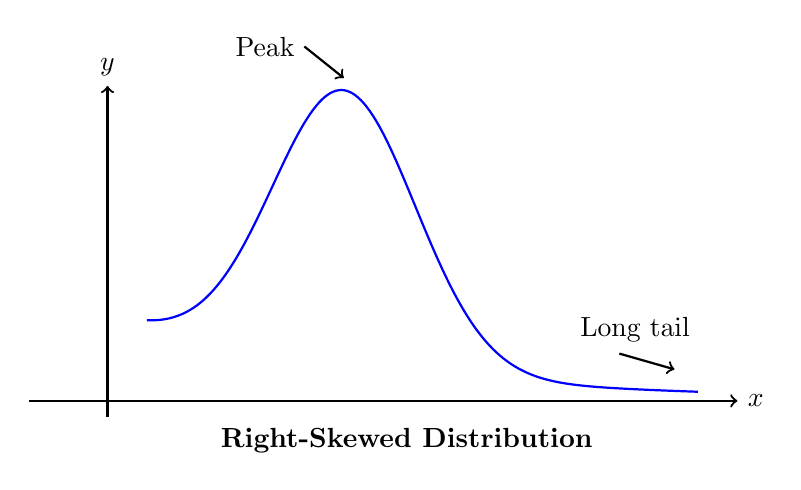
\begin{tikzpicture}
  \draw[thick, ->] (-1,0) -- (8,0) node[right] {$x$};
  \draw[thick, ->] (0,-0.2) -- (0,4) node[above] {$y$};

  \draw[thick, blue, smooth, samples=100, domain=0.5:7.5] 
    plot (\x, {3.5*exp(-0.6*(\x - 3)^2) + 0.6*exp(-0.3*(\x - 2))});
    
  \node at (3.8,-0.5) {\textbf{Right-Skewed Distribution}};    

  \node at (2,4.5) {Peak};
  \draw[->, thick] (2.5,4.5) -- (3,4.1);

  \node at (6.7,0.9) {Long tail};
  \draw[->, thick] (6.5,0.6) -- (7.2,0.4);
\end{tikzpicture}
\end{center}
\caption{An illustration of a right (positive) skewed distribution}
\end{figure}

\end{document}